\documentclass{article}
\usepackage{graphicx}
\usepackage{hyperref}
\usepackage{xcolor}
% Here: H option for float placement
\usepackage{float}

% caption and subcaption work together
\usepackage{subcaption} % loads the caption package

\graphicspath{ {images/} }

\begin{document}
\pagecolor{white}

\title{%
  Implementation and evaluation of Learning Algorithms in Python
  \large \\HWI - ML Sapienza}

\author{Giulio Serra 1904089}
\date{November 10, 2019}

\maketitle

\begin{titlepage}
\end{titlepage}

\tableofcontents

\begin{titlepage}
\end{titlepage}


\section{Introduction}\label{sec:intro}
This essay will describe the implementation of two learning algorithm using Python and the Sklearn library, evaluating the performances based on the accuracy of the prediction , varying some parameters such as features and dataset.

\section{Understanding the Classification Problem}
The aim of this implementation is to train two learning algorithms to recognize instructions parsed from a file, by categorizing them by High and Low type and by Compliler.\\
So it's a problem of text classification: each new instruction need to be categorized and then the model will autonomusly put new words in one of the categories once is trained.\\In the fist case, we have a binary classifier(each instruction could be categorize only in high or low), while in the second scenario we have three possible types of instructions: GCC, ICC and CLANG, so we are talking about a multiclass classsifier.


\section{Learning Algorithms}\label{sec:intro}

A learning algorithm can predict the value of an input set of data within an acceptable range, generally speaking, more data is feed to the algorithm, higher the accuracy of the algorithm increase.\\\\
Having two set of data X(input data) and Y(expected values) a learning algorithm can compute a function h(x) (hypothesis function) that is more or less similar to the original function f(x) = y that h(x) tries to mimic.\\\\
In order to train the learning algorithm, we have to produce a set of data (rappresenting a sample of all the possible values of the X set), than divide it into two sub-sets:a train set and test set, the train set is used to train the algorithm, to predict the correct values given x inputs.The test set on the other hand, has the purpose to validate the predictions of a learning algorithm once is trained.\\\\
The same needs to be done to the Y set that needs to be splitted between test and train set.\\

\subsection{Decision Tree}\label{sec:decTree}

The Decision Tree is a supervised learning algorithm that creates a tree based on conjunctions of disjunctions that leds to positive results.\\\\
Each node of the Decision Tree rappresent an attribute of the tuple of the dataset, each branch rappresent a decision(possible value of the tuple), after a certain number of decisions we eventually get an outcome.

\subsection{Multinomial Naive Bayes }\label{sec:multnaiveBayes}
The multinomial Naive Bayes Classifier is a supervised learning algorithm that belongs to a family of probabilistic classifiers based on the Bayes Rule, it works by assigning lables to the problem instances using vectors of features values, using the maximum likelIhood(MLE) by estimating the parameters of a probabilistic distributions.


\section{Implementations in Python}\label{sec:intro}
The two learning algorithm are part of the python Sklearn library: in order to implement and train the algorithm we have to first parse the data inside the \verb|train_dataset.json| file, then we need to sort all the data by category in a CSV file, in order to train and test our model.

\subsection{Parsing the Train Set}
As we said, the jsonl need to be parsed and converted in a CSV in order to train our model, this can be achieved by parsing the file line-by-line:\\

\begin{verbatim}
if not os.path.isfile(input_path):
       print("File path {} does not exist. Exiting...".format(filepath))
        
inputFile = open(input_path,'r');
outputFile = open(output_path,'w');

line=inputFile.readline()
output = csv.writer(outputFile,delimiter='\t')

while line:
    data = json.loads(line)
    instr=""
    count=0
    for command in data["instructions"]:
        if command.split(" ")[0][0]=='m':
            count+=1
        instr=instr+command+","
    output.writerow([  instr,count,data["opt"],data["compiler"], len(instr.split(" "))])
    line = inputFile.readline()

inputFile.close() #close the input file
outputFile.close()#close the output csv file
\end{verbatim}
Then we can create our db of instructions to feed to our model:
\begin{verbatim}
filename ='train_datasetCSV.csv'
db = pd.read_csv(filename, sep='\t', header=None, 
names=['instructions','mov', 'opt','compiler','LOC'], 
dtype={'mov': np.int32, "LOC": np.int32})
\end{verbatim}

\subsection{Vectorizing the Data}
In order to efficiently train our models is not enough to feed them the raw files, we need to vectorize them.We can apply various strategies to achieve it: for example we can use the Count Vectorizer method that assign to each word in the vocabulary a token to feed to the machine learning algorithm.\\
Another vectorizer known as Tf-idf Vectorizer, count the occurencies of each words inside the documents and lastly we have Count Vectorizer combined with n-grams, that check chunks of 1 to n words, instead of building the vocabulary word-by.word.\\Here is the implementation:\\

\begin{verbatim}
def countVectorizer(db):
    
    start_time = time.time()

    x=[]
    y=[]
    x_new=[]
    
    for ins in db.instructions:
        temp=ins.split(",")
        s=""
        for cmd in temp:
            s=s+cmd.split(" ")[0]+" "
        x_new.append(s)
        
    vectorizer = CountVectorizer(stop_words=None)
    x = vectorizer.fit_transform(x_new)
    y = db.opt
    
    X_train, X_test, y_train, y_test = train_test_split(x, y,
                                                    test_size=0.3)
    print("Count vectorizer:")
    print("Train: %d - Test: %d" %(X_train.shape[0],X_test.shape[0]))
    elapsed_time = time.time() - start_time
    print("Vectorizer elapsed Time: %.3fs" %elapsed_time)
    print("\n")
    return  X_train, X_test, y_train, y_test

countVectorizer(db)

def tfidfVectorizer(db):
    
    start_time = time.time()
    
    x=[]
    y=[]
    x_new=[]
    
    for ins in db.instructions:
        temp=ins.split(",")
        s=""
        for cmd in temp:
            s=s+cmd.split(" ")[0]+" "
        x_new.append(s)
        
    vectorizer=TfidfVectorizer()
    x = vectorizer.fit_transform(x_new)
    y = db.opt

    X_train, X_test, y_train, y_test = train_test_split(x, y,
                                                    test_size=0.3)
    print("tfidfVectorizer:")
    print("TrainSet: %d - TestSet: %d" %(X_train.shape[0],X_test.shape[0]))
    elapsed_time = time.time() - start_time
    print("TfidfVectorizer elapsed Time: %.3fs" %elapsed_time)
    print("\n")
        
    return  X_train, X_test, y_train, y_test

tfidfVectorizer(db)

def vectorizer2Gram(db):
    
    start_time = time.time()
    
    vectorizer = CountVectorizer(ngram_range=(2,2)) # multinomial
    x = vectorizer.fit_transform(db.instructions)
    y = db.opt
    
    X_train, X_test, y_train, y_test = train_test_split(x, y,
                                                    test_size=0.3)
    print("vectorizer2Gram:")
    print("TrainSet: %d - TestSet: %d" %(X_train.shape[0],X_test.shape[0]))
    elapsed_time = time.time() - start_time
    print("vectorize2Gram elapsed Time: %.3fs" %elapsed_time)
    print("\n")
        
    return  X_train, X_test, y_train, y_test

vectorizer2Gram(db)
\end{verbatim}

\subsection{Splitting the DataSet}
Taking a closer look to the execution of a vectorization, we can see that the DataSet is not evenly splitted, that's because giving more data to the train set makes the learning algorithm more precise:

\begin{verbatim}
tfidfVectorizer:
TrainSet: 21000 - TestSet: 9000
TfidfVectorizer elapsed Time: 11.012s
\end{verbatim}

\subsection{Creating the Model and Processing the Data}
Now that we have the vectorized data ready, we can feed them to a learning algorithm, here is the implementation of the most efficient combination between vectorization and learning algorithm:\\

\begin{verbatim}

def DecisionTreeOPT():
    
    start_time = time.time()
        
    print("DecisionTree - countVectorizer")
    
    xTrain, xTest, yTrain, yTest=countVectorizer(db)
    
    model = DecisionTreeClassifier(random_state=0).fit(xTrain, yTrain)
    yPred = model.predict(xTest)
    
    print("confusion Matrix of DT/ cVectorizer:\n")
    print(confusion_matrix(yTest, yPred))
    print("\n")
    print("classificationReport Matrix of DT/ cVectorizer:\n")
    print(classification_report(yTest, yPred))
    
    plotPrecisionRecallOPT(yTest,yPred,"DecisionTree - countVectorizer")
    
    elapsed_time = time.time() - start_time
    print("elapsed Time: %.3fs" %elapsed_time)
    print("-------------------------------------------")
    
    print("DecisionTree - tfidfVectorizer")
    
    xTrain, xTest, yTrain, yTest=tfidfVectorizer(db)
    
    model = DecisionTreeClassifier(random_state=0).fit(xTrain, yTrain)
    yPred = model.predict(xTest)
    
    print("confusion Matrix of DT/ tfidfVectorizer:\n")
    print(confusion_matrix(yTest, yPred))
    print("\n")
    print("classificationReport Matrix of DT/ tfidfVectorizer:\n")
    print(classification_report(yTest, yPred))
    
    plotPrecisionRecallOPT(yTest,yPred,"DecisionTree - tfidfVectorizer")
    
    elapsed_time = time.time() - start_time
    print("elapsed Time: %.3fs" %elapsed_time)
    print("-------------------------------------------")

    print("DecisionTree - vectorizer2Gram")
    
    xTrain, xTest, yTrain, yTest=vectorizer2Gram(db)
    
    model = DecisionTreeClassifier(random_state=0).fit(xTrain, yTrain)
    yPred = model.predict(xTest)
    
    print("confusion Matrix of DT/ vectorizer2Gram:\n")
    print(confusion_matrix(yTest, yPred))
    print("\n")
    print("classificationReport Matrix of DT/ vectorizer2Gram:\n")
    print(classification_report(yTest, yPred))
    
    plotPrecisionRecallOPT(yTest,yPred,"DecisionTree - vectorizer2Gram")
    
    elapsed_time = time.time() - start_time
    print("elapsed Time: %.3fs" %elapsed_time)
    print("-------------------------------------------")
    
DecisionTreeOPT()
\end{verbatim}

\section{Evaluating the Perfomances}
The most critical aspect of every learning algorithm while approaching a text classification problem, is of course the ability to correctly predict the category where a text or a word will fit in: this paragraph will describe all the criteria used to evaluate all the different combination of vectorization an learning algorithms:

\subsection{Precision}
The precision of the learning algorithm measure the proportion of the postives that was correctly identified, as the formula suggest:\\\\	
 
 \begin{center}
$Precision =\frac{TP}{TP+FP}. $
\end{center}
The precision rappresent the rateo between true positive(positive classified correctly by the algorithm) and the sum of true positive and false positive(positive wrongly classified as such).

\subsection{Recall}
The recall measure the percentage of actual positive correctly predicted by the algorithm, so we can define recall as follow:

  \begin{center}
$Recall =\frac{TP}{TP+FN}. $
\end{center}
To measure how good is a learning algorithm is, we have to measure both the recall and the accuracy, usually incrementing one come to the expense of the other.\\

\subsection{F1 Score}
The F1 score is the indicator of a test accuracy: it considers both precision and recall to compute the score:\\

  \begin{center}
 $F1 =2\times \frac{precision\times recall}{precision+recall}. $
 \end{center}
 \clearpage
So here is a classification report 
(obtained by the command \verb|classification_report(yTest, yPred)|) of the best combination(in terms of performances) of the vectorizer2gram ad Decision Tree learning algorithm (Binary classifier scenario):\\
 
 \begin{verbatim}
 classificationReport Matrix of DT/ vectorizer2Gram:

              precision    recall  f1-score   support

           H       0.80      0.80      0.80      3609
           L       0.86      0.86      0.86      5391

    accuracy                           0.84      9000
   macro avg       0.83      0.83      0.83      9000
weighted avg       0.84      0.84      0.84      9000
 \end{verbatim}

\subsection{The Precision-Recall curve}
Beside looking to the precision and recall values themself, we can plot an usefull graph that helps evaluate performances between learning algorithms: it's the precision-recall curve.\\
The PR curve plot the precision on the X axis and the recall on the Y axis, it measures the trade-off between the true positive rate and the positive predictive value for a predictive model, using different probability thresholds, here are two executions for the binary classification problem(High and Low instructions) for a good and a bad learning algorithm:

\begin{figure}[h]
\centering
\subcaptionbox{Good Learning Algorithm}{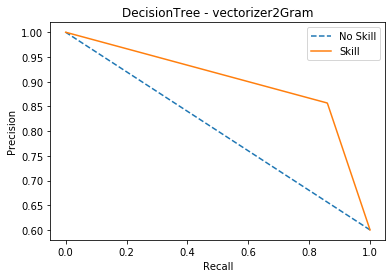
\includegraphics[width=0.45\textwidth]{images/good_alg}}%
\hfill % <-- Seperation
\subcaptionbox{Bad Learning Algorithm}{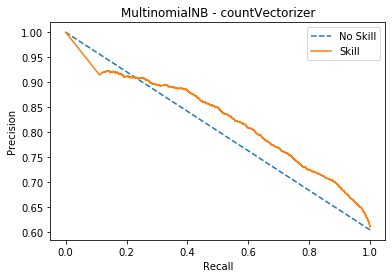
\includegraphics[width=0.45\textwidth]{images/bad_alg}}%
\caption{PR curve of two learning algorithm}
\end{figure}

The difference lies in the curve being below or over the no-skill line, basically the algorithm in figure(b) has less probability of correctly categorizing a word than randomly putting in a category.
\clearpage
Here is the equivalent curve for a multiclass learning algorithm:
  \begin{figure}[h]
\centering
\subcaptionbox{Good Learning Algorithm}{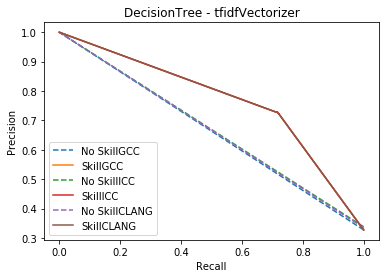
\includegraphics[width=0.45\textwidth]{images/good_multiclass_algorithm}}%
\hfill % <-- Seperation
\subcaptionbox{Bad Learning Algorithm}{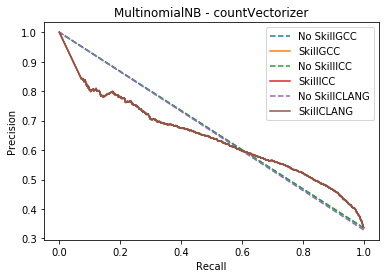
\includegraphics[width=0.45\textwidth]{images/bad_multiclass_alg}}%
\caption{PR curve of two multiclass learning algorithm}
\end{figure}

\section{BlindTest}
Once we evaluated the best combination of vectorization and learning algorithm for both the binary classification problem and multiclass, we need to evaluate how they would react  
to a different set of data once they are trained.\\

\subsection{Binary Classification Problem}
So the first thing to do is to parse the \verb|test_dataset_blind.jsonl| :\\

\begin{verbatim}
if not os.path.isfile(input_path_blind):
       print("File path {} does not exist. Exiting...".format(filepath))
        
inputFile = open(input_path_blind,'r');
line=inputFile.readline()

blind_test_data = [];
while line:
    data = json.loads(line)
    instr=""
    for command in data["instructions"]:
        instr = instr + command+", "
        
    blind_test_data.append(instr)
    line = inputFile.readline()
    
print(len(blind_test_data))
\end{verbatim}

Now it's time to train back the most efficients algorithms(bynary and multiclass):

\begin{verbatim}
model,vectorize = DecisionTreeOPT() #training with csv file

x_blind_test = vectorize.transform(blind_test_data)
y_pred = model.predict(x_blind_test)

low_instr=0.0
high_instr=0.0

for i in y_pred:
    if(i=="L"):
        low_instr+=1;
    else:
        high_instr+=1;

db_length = len(y_pred);

lPerc = (low_instr/db_length)*100;
hPerc = (high_instr/db_length)*100;
        
print("LOW=%.6f HIGH=%.6f" %(lPerc,hPerc));

classificationReport Matrix of DT/ vectorizer2Gram:

              precision    recall  f1-score   support

           H       0.79      0.77      0.78      3636
           L       0.85      0.86      0.86      5364

    accuracy                           0.83      9000
   macro avg       0.82      0.82      0.82      9000
weighted avg       0.83      0.83      0.83      9000

elapsed Time: 155.786s

\end{verbatim}
So here is the output for the reading of just the CSV file:
\begin{center}
\begin{verbatim}
LOW=59.746667 HIGH=40.253333
\end{verbatim}
\end{center}
And here is the percentage categorizing the BlindSet:
\begin{center}
\begin{verbatim}
LOW=58.866667 HIGH=41.133333
\end{verbatim}
\end{center}
So the algorithm just missclassified only a small fraction of LOW and HIGH instructions.\\


\subsection{Multiclass Classification Problem}
Again, we have to do the same thing for the multiclass learning problem:\\

\begin{verbatim}
model,vectorize = DecisionTreeCompiler()

x_blind_test = vectorize.transform(blind_test_data)
y_pred = model.predict(x_blind_test)

gcc_instr=0.0
icc_instr=0.0
clang_instr =0.0

for i in y_pred:
    if(i=="gcc"):
        gcc_instr+=1;
    elif(i=="icc"):
        icc_instr+=1;
    else:
        clang_instr+=1;

db_length = len(y_pred);

gccPerc = (gcc_instr/db_length)*100;
iccPerc = (icc_instr/db_length)*100;
clangPerc = (clang_instr/db_length)*100;

print("GCC=%.6f ICC=%.6f CLANG=%.6f" %(gccPerc ,iccPerc,clangPerc));

classificationReport Matrix of DT/ vectorizer2Gram:

              precision    recall  f1-score   support

       clang       0.92      0.91      0.91      3001
         gcc       0.90      0.91      0.90      2978
         icc       0.93      0.92      0.92      3021

    accuracy                           0.91      9000
   macro avg       0.91      0.91      0.91      9000
weighted avg       0.91      0.91      0.91      9000

elapsed Time: 116.865s

\end{verbatim}
The original content of the DataSet were three equally diveded set of GCC , ICC and CLANG set of instructions:
\begin{verbatim}
GCC=33.333333 ICC=33.333333 CLANG=33.333333
\end{verbatim}
And here is the output of the learning algorithm using the blind data set:
\begin{verbatim}
GCC=33.866667 ICC=33.366667 CLANG=32.766667
\end{verbatim}
Again the classifier just misclassified only a small fraction of the instructions, those result are compatible both with the the 0.91 accuracy of the report matrix and the precision-recall curve.

\section{References}
	The Scikit-learn library for Python: \url{https://scikit-learn.org/stable/}\\\\
	The Precision-Recall curve in Python using Scikit-learn: \url{https://scikit-learn.org/stable/auto_examples/model_selection/plot_precision_recall.html}

\end{document}

